\color{black}
\subsection{Specifica componenti Romeo::Model::Help}
\label{specificaHelp}

	\begin{figure}[!h]
				\centering
				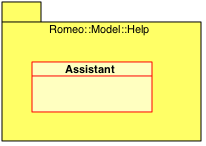
\includegraphics[scale=1.00]{../Specifica_Tecnica/Content/Immagini/Help.png}
				\caption{Diagramma package \textsl{Romeo::Model::Help}}
				\label{comp_romeo::model::help}
	\end{figure}
	
Package\g{} che contiene la classe che si occupa della gestione logica della guida utente.
	%%%%%%%%%%%%%%%%%%%%
	%     CLASSE HELP
	%%%%%%%%%%%%%%%%%%%%%%%
	\subsubsection{Assistant (class)}
	\label{spehelp}
	\begin{figure}[!h]
	\centering
				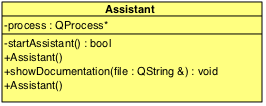
\includegraphics[width=0.6\linewidth]{./Content/Immagini/model/Assistant.png}
				\caption{Diagramma classe \textsl{Assistanti}}
				\label{cl_log}
	\end{figure}

	\paragraph{Descrizione:\\}
	 Classe che rappresenta il processo Qt Assistant, utilizzato per la gestione della guida utente.
	
	\paragraph{Utilizzo\\} 
	Viene utilizzata per gestire la richiesta dell'utente, che vuole visualizzare una determinata pagina all'interno della guida utente.
					
	\paragraph{Eredita da:}
		\begin{itemize}
			\item Qt::QProcess
		\end{itemize}
	
	\paragraph{\color{black}Attributi \\}
		\begin{itemize}
			\item \color{teal} \verb!- process : QProcess *!\\
				   	\color{black}
				   	\subparagraph{Descrizione:} puntatore al processo esterno Qt Assistant.
		\end{itemize}
		
	\paragraph{\color{black}Metodi\\}
		\begin{itemize}
			\item \color{blue} \verb!+ Assistant()!\\
							 \color{black}
							 \subparagraph{Descrizione:} costruttore per un oggetto di tipo \textsl{Assistant}.
							 
			\item  \color{blue} \verb!- startAssistant() : boolean!\\
					\color{black}
					\subparagraph{Descrizione:} metodo che controlla se il processo esterno associato a Qt Assistant è già attivo, in caso negativo si preoccupa di farlo partire. 
					\\Ritorna un booleano per indicare se il processo è attivo o no.
					
			\item \color{blue} \verb!+ showDocumentation(file : const QString &) : void!\\
					 \color{black}
					 \subparagraph{Descrizione:} metodo che si occupa di visualizzare nell'help di Qt Assistant la pagina \verb!HTML! passata come argomento.\\
					 \subparagraph{Argomenti}
						\begin{itemize}
							\item \color{RoyalPurple} \verb!file : const QString &!\\
							\color{black}Rappresenta il path della pagina \verb!HTML! da visualizzare nell'help di Qt Assistant.
						\end{itemize}
		\end{itemize}
	
	
